\documentclass[12pt,a4paper]{article}

% Packages
\usepackage{
    amsmath,
    amssymb,
    graphicx,
    titletoc,
    fancyhdr,
    geometry,
    babel,
    xcolor,
    enumerate,
    fix-cm,
    tocbibind,
    listings,
    float,
    enumitem,
    subcaption,
    hyperref
}

% Define colors
\definecolor{vgreen}{RGB}{104,180,104}
\definecolor{vblue}{RGB}{49,49,255}
\definecolor{vorange}{RGB}{255,143,102}

% Listings customization
\renewcommand\lstlistingname{Figura}
\renewcommand\lstlistlistingname{Figura}

\makeatletter
\newcommand*\@lbracket{[}
\newcommand*\@rbracket{]}
\newcommand*\@colon{:}
\newcommand*\colorIndex{%
    \edef\@temp{\the\lst@token}%
    \ifx\@temp\@lbracket \color{black}%
    \else\ifx\@temp\@rbracket \color{black}%
    \else\ifx\@temp\@colon \color{black}%
    \else \color{vorange}%
    \fi\fi\fi
}
\makeatother

% Setup for listings
\lstset{
    captionpos=b,
    belowcaptionskip=\bigskipamount,
    frame=single,
    basicstyle=\small\ttfamily,
    numbers=left,
    numberstyle=\tiny\color{gray},
    xleftmargin=2em,
    framexleftmargin=2em,
    backgroundcolor=\color{vgreen!10},
    stepnumber=1,
    showstringspaces=false,
    keywordstyle=\color{vblue},
    commentstyle=\color{gray},
    stringstyle=\color{vorange},
}

\begin{document}

\begin{titlepage}
    \centering
    
\includegraphics[scale=1]{M2_Modelos_de_Programación/reporte/figuras/Logo_Tec.png}\\
    \vspace{.5cm}
    \bfseries\large Escuela de Ingeniería y Ciencias
        
    \vspace{5cm}
    \centering
    \textbf{\Huge Cómputo en la Nube}
    \vspace{0.5cm}
        
    {\Large Creación de Máquinas Virtuales en la Nube}

    \vspace{5cm}
        
    \textbf{\LARGE Armando Bringas Corpus}
        
    \vspace{0.5cm}
        
    {\large A01200230}
        
    \vfill
        
\end{titlepage}

\section{Introducción}

El propósito de la siguiente práctica es utilizar dos de los servicios más comunes de cómputo en la nube, Microsoft Azure y Google Cloud para la creación de Máquinas Virtuales en la nube. En una práctica pasada se estuvo experimentando con la creación de las mismas en un entorno local, sin embargo, en esta ocasión se realzará en los servicios anteriormente mencionados con los cuales se estarán analizando algunas ventajas y desventajas de dichas plataformas.

\section{Máquina Virtual Azure}

\subsection{Creación de la Máquina Virtual de Azure}

El primer paso es la creación de la máquina virtual en Microsoft Azure con la cual se estará sacando provecho de la cuenta de Azure Student para su creación. En este caso seleccionamos la Máquina Virtual menos costosa y económica con respecto a los recursos que estará consumiendo.

\begin{figure}[H]
    \centering
    \includegraphics[width=.65\linewidth]{M4_Servicios_Cómputo_en_la_Nube/Tarea_5_Creación_Máquinas_Virtuales_en_Nube/reporte/figuras/1_1_1_Creación_MV_Azure.png}
    \captionof{lstlisting}{Creación de la Máquina Virtual en Azure}
    \label{fig:Azure_1}
\end{figure}

La figura \ref{fig:Azure_2} muestra el costo de nuestra Máquina Virtual por hora, de igual manera al momento de configurarla se seleccionó los puertos de entrada \textit{HTTP, HTTP y SSH} para permitir que la Máquina Virtual sea accesible a trabes de la red de Internet pública. Se estableció un usuario y contraseña para poder acceder a la misma.

\begin{figure}[H]
    \centering
    \includegraphics[width=1\linewidth]{M4_Servicios_Cómputo_en_la_Nube/Tarea_5_Creación_Máquinas_Virtuales_en_Nube/reporte/figuras/1_1_2_Creación_MV_Azure.png}
    \captionof{lstlisting}{Creación de la Máquina Virtual en Azure}
    \label{fig:Azure_2}
\end{figure}

\vspace{1em}

Una vez validada la información para la creación de la Máquina Virtual se procedió con la creación de la nueva MV como se ve en la figura \ref{fig:Azure_3} con la cual nos cercioramos que su implementación fuera completada y exploramos el recurso para poder obtener su dirección externa IP, en este caso fue la \textbf{40.121.223.205}.

\begin{figure}[H]
    \centering
    \includegraphics[width=1\linewidth]{M4_Servicios_Cómputo_en_la_Nube/Tarea_5_Creación_Máquinas_Virtuales_en_Nube/reporte/figuras/1_1_3_Creación_MV_Azure.png}
    \captionof{lstlisting}{Creación de la Máquina Virtual en Azure}
    \label{fig:Azure_3}
\end{figure}

\subsection{Instalación de PHP y el servidor Web}

Posteriormente se instaló la aplicación de Bitvise el cual es gratuito y funciona como un cliente SSH el cual nos permite conectarnos a través de una consola a la Máquina Virtual para la transferencia de archivos. Como se observa en la figura \ref{fig:Azure_4} se configuro el host con la dirección \textbf{40.121.223.205}, puerto \textbf{22} y el usuario y contraseño que se definieron en la creación de la Máquina Virtual para establecer la conexión.

\begin{figure}[H]
    \centering
    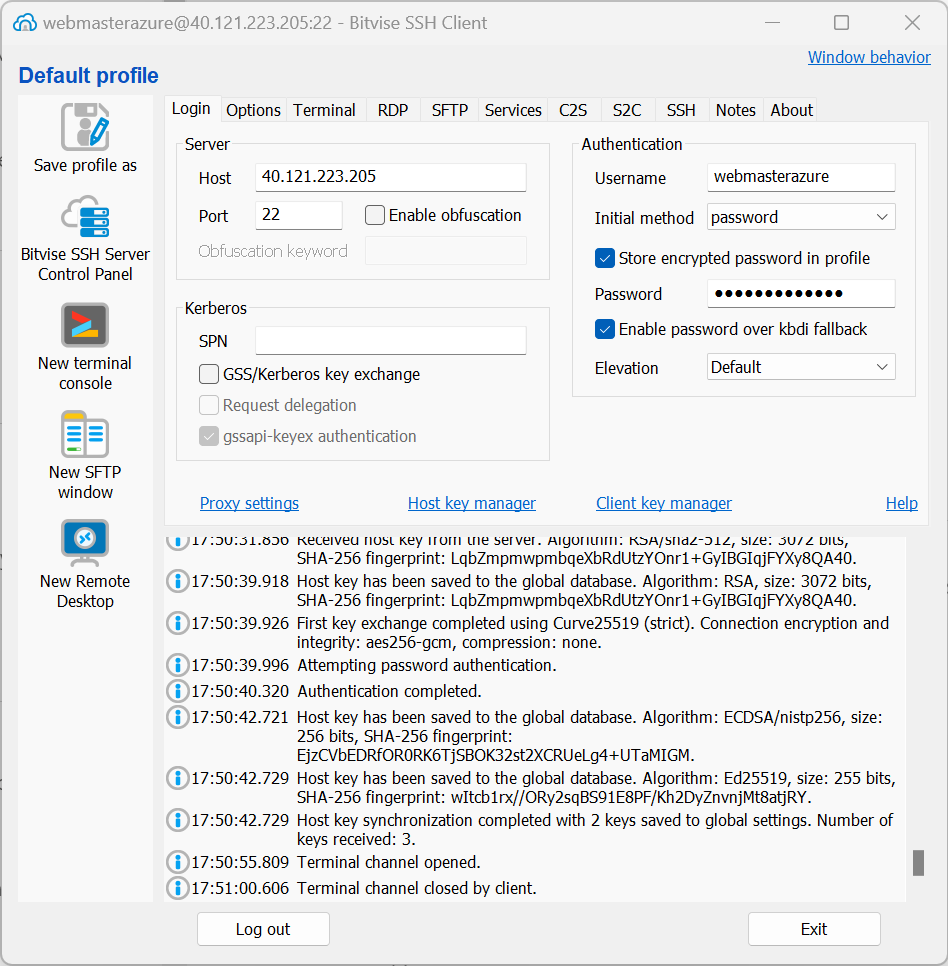
\includegraphics[width=1\linewidth]{M4_Servicios_Cómputo_en_la_Nube/Tarea_5_Creación_Máquinas_Virtuales_en_Nube/reporte/figuras/1_2_1_PHP_servidor_Web.png}
    \captionof{lstlisting}{Configuración de Bitvise}
    \label{fig:Azure_4}
\end{figure}

Al momento de establecer la conexión se abrió una consola con la cual procedimos a ingresar los siguientes comandos de Linux:

\begin{itemize}
    \item \textbf{sudo su - root}: para cambiarnos al entorno de súper usuario.
    \item \textbf{apt update}: para actualizar las aplicaciones dentro de la Máquina Virtual.
    \item \textbf{apt -y install apache2}: para la instalación del servidor web apache2    
\end{itemize}

Finalmente, para verificar el funcionamiento del servidor web ejecutamos el comando \textbf{service apache2 status}, como se puede ver en la figura \ref{fig:Azure_5} su funcionamiento es el esperado ya que se encuentra activo.

\begin{figure}[H]
    \centering
    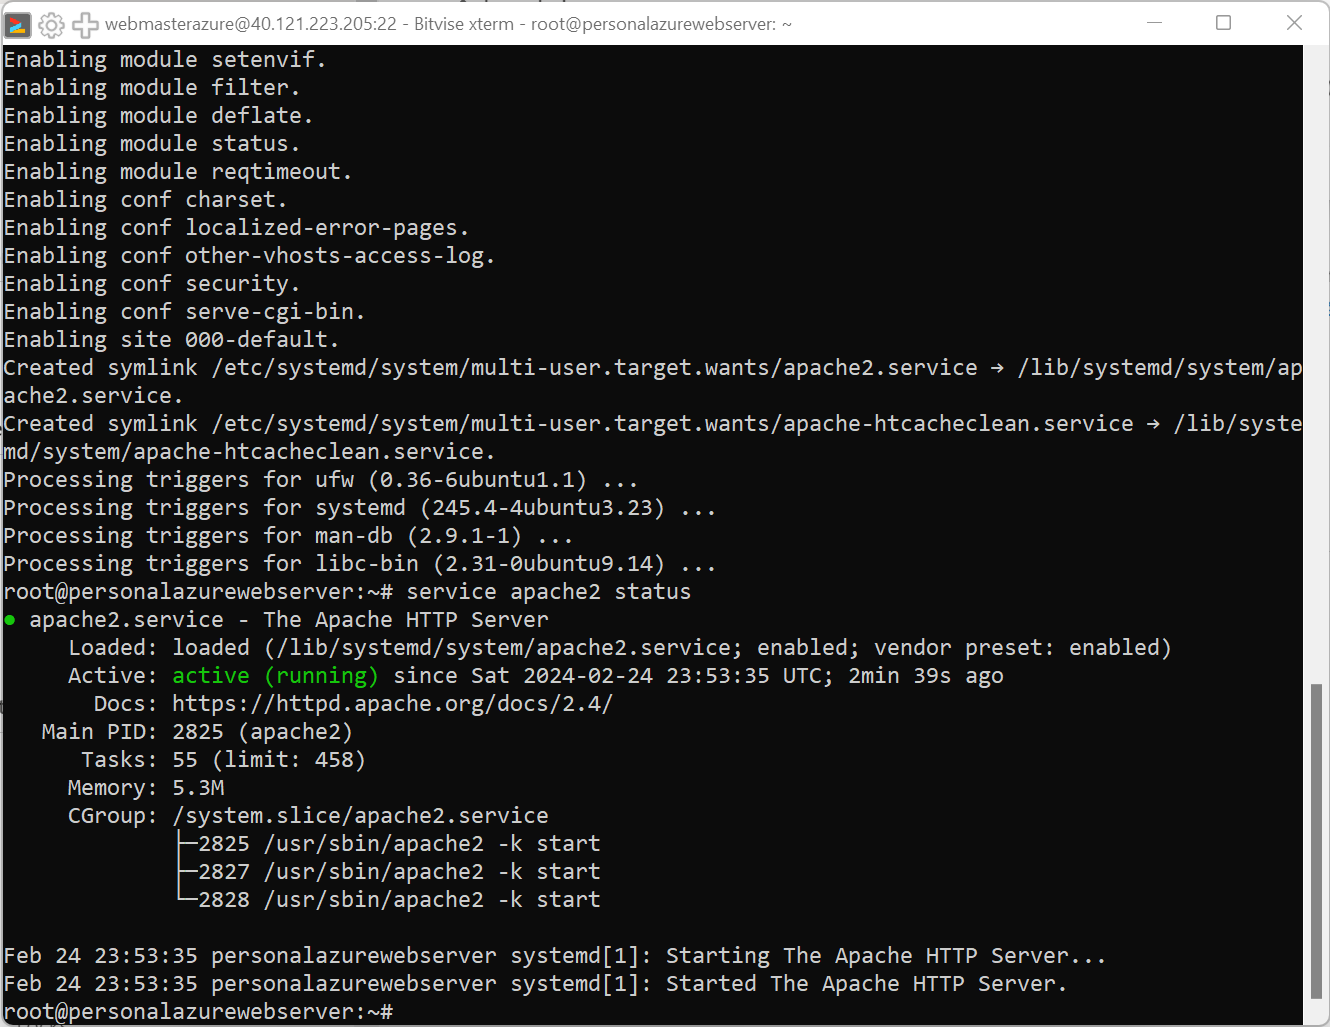
\includegraphics[width=1\linewidth]{M4_Servicios_Cómputo_en_la_Nube/Tarea_5_Creación_Máquinas_Virtuales_en_Nube/reporte/figuras/1_2_2_PHP_servidor_Web.png}
    \captionof{lstlisting}{Configuración del servidor web apache2}
    \label{fig:Azure_5}
\end{figure}

Finalmente se ejecutó el comando \textbf{chmod 777 /var/www/html} para permitir la transferencia de archivos al servidor web.

\subsection{Configuración de la Máquina Virtual para que sea pública}

Como establecimos en la configuración de la Máquina Virtual con la habilitación de los  puertos de entrada \textit{HTTP, HTTP y SSH} para poder ingresar al servidor web por medio de cualquier navegador público, en la siguiente figura \ref{fig:Azure_6} podemos obervar que accedemos al mismo por medio de la dirección IP \textbf{40.121.223.205}.

\begin{figure}[H]
    \centering
    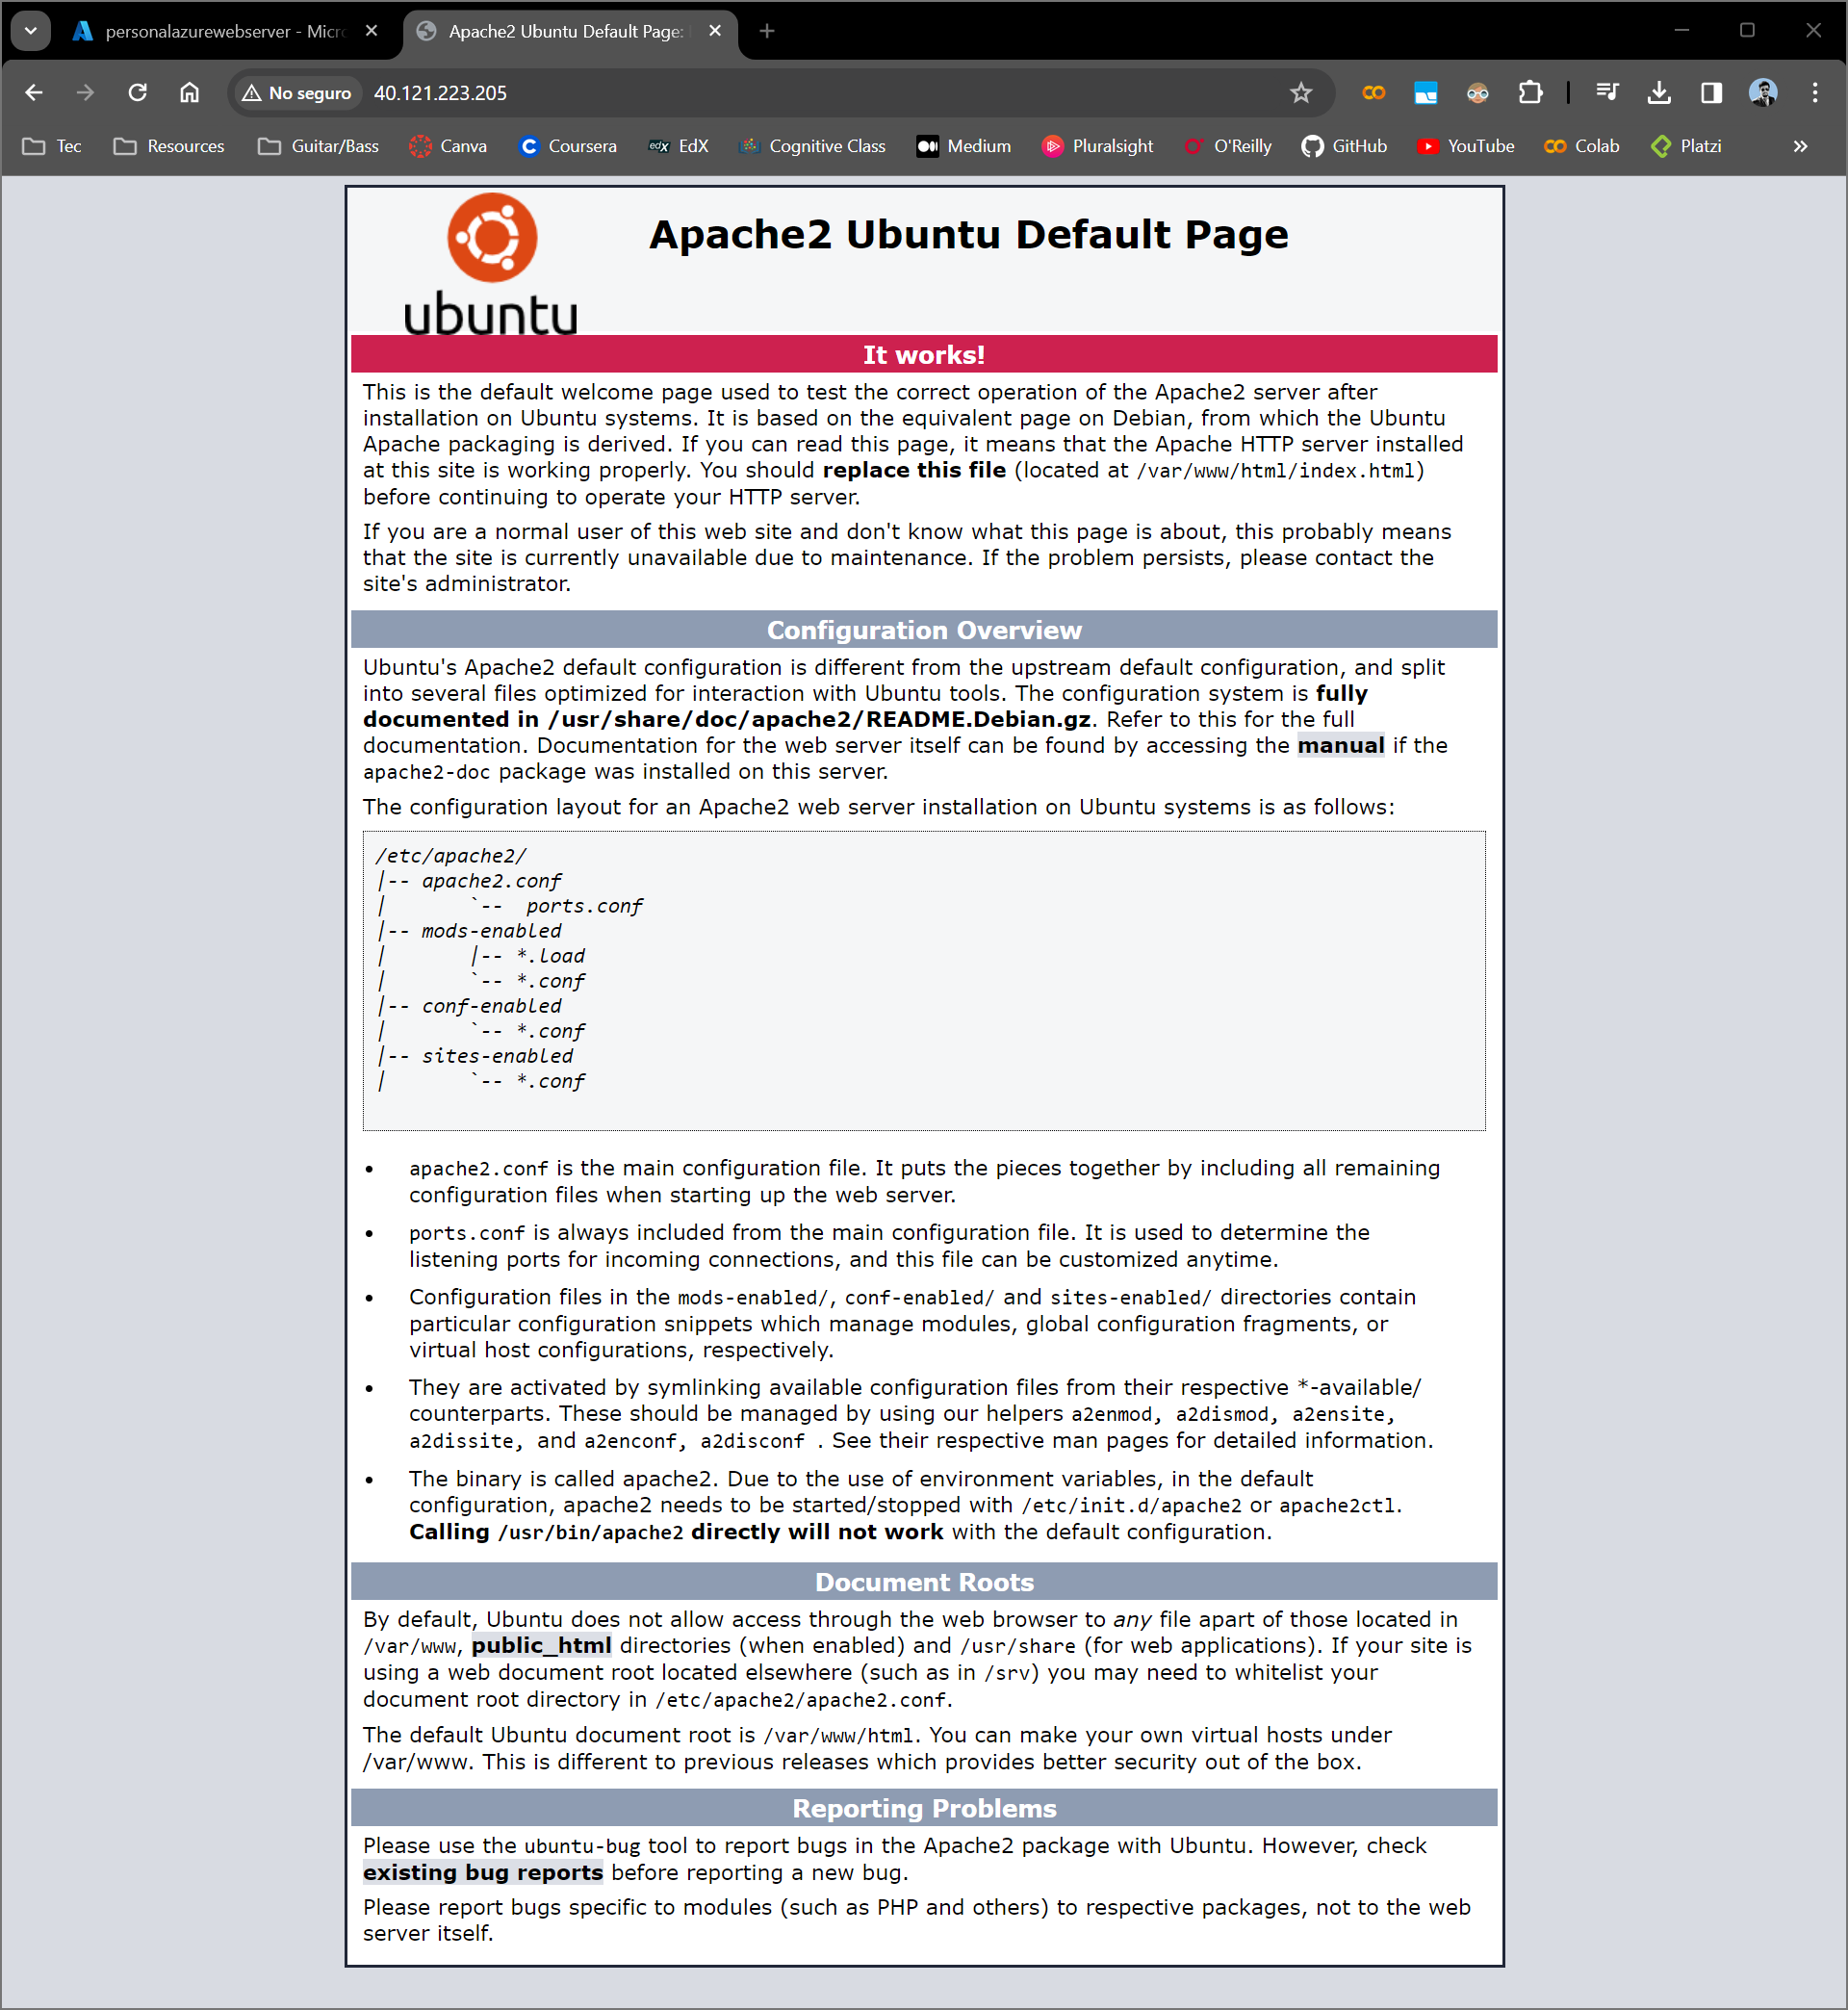
\includegraphics[width=1\linewidth]{M4_Servicios_Cómputo_en_la_Nube/Tarea_5_Creación_Máquinas_Virtuales_en_Nube/reporte/figuras/1_3_1_Configuración_Pública.png}
    \captionof{lstlisting}{MV como servidor web, página de apache por defecto}
    \label{fig:Azure_6}
\end{figure}

\subsection{Carga de los archivos del sitio}

Con la aplicación de Bitvise establecemos una conexión \textbf{SFTP} para permitir la transferencia de archivos y de esta manera cargamos los archivos de nuestro sitio web que queremos dessplegar como se ve en la figura \ref{fig:Azure_7}.

\begin{figure}[H]
    \centering
    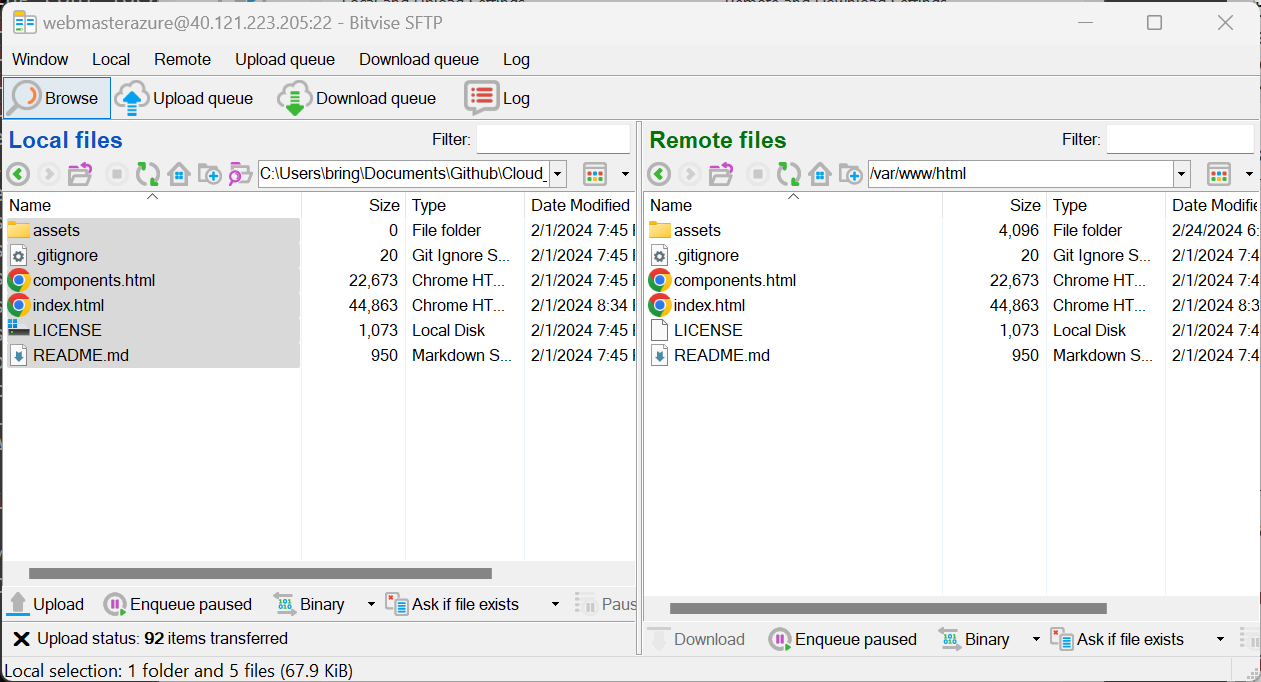
\includegraphics[width=1\linewidth]{M4_Servicios_Cómputo_en_la_Nube/Tarea_5_Creación_Máquinas_Virtuales_en_Nube/reporte/figuras/1_4_1_Carga_archivos.png}
    \captionof{lstlisting}{Transferencia de archivos a la Máquina Virtual}
    \label{fig:Azure_7}
\end{figure}

\vspace{25em}

Finalmente ingresamos a la dirección IP textbf{40.121.223.205} a través de una ventana de incógnito y corrobaramos así que el sitio web que se visualiza fue el que cargamos en la Máquina Virtual, de esta manera corroboramos que la creación de la Máquina Virtual y su configuración fue exitosa.

\begin{figure}[H]
    \centering
    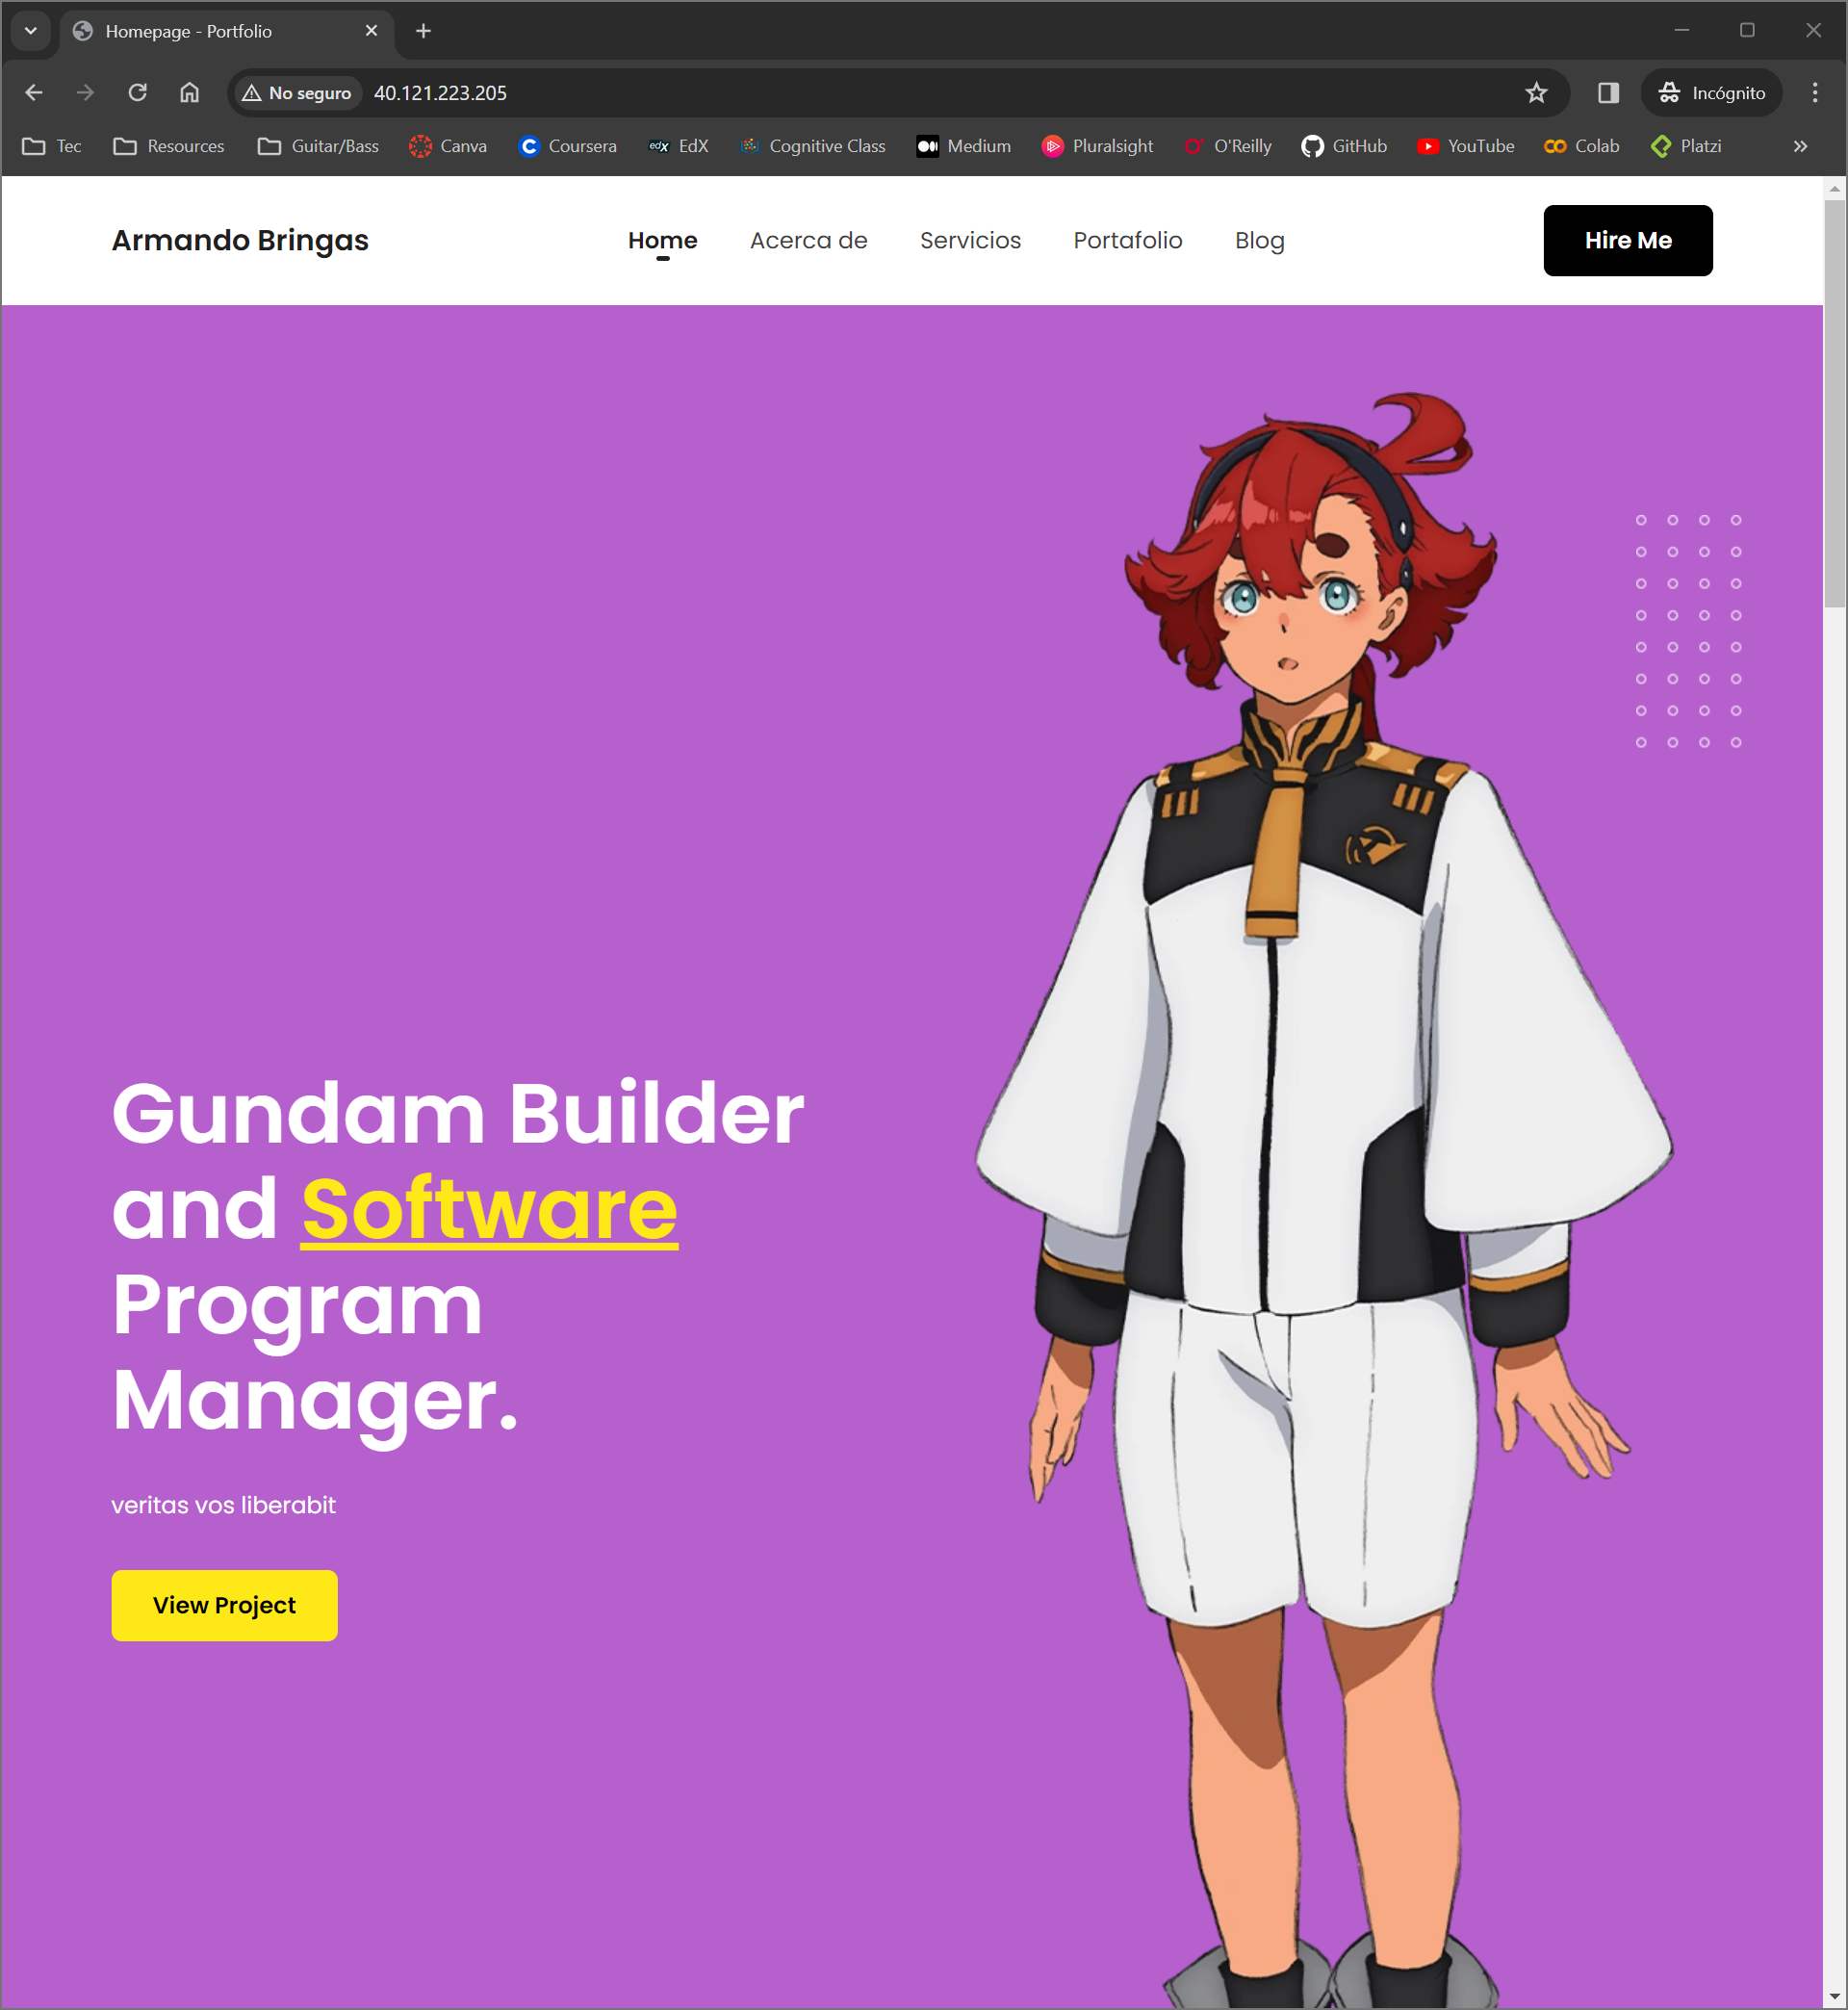
\includegraphics[width=1\linewidth]{M4_Servicios_Cómputo_en_la_Nube/Tarea_5_Creación_Máquinas_Virtuales_en_Nube/reporte/figuras/1_4_2_Carga_archivos.png}
    \captionof{lstlisting}{Visualización del sitio web}
    \label{fig:Azure_8}
\end{figure}

\section{Máquina Virtual Google}

\subsection{Creación de la Máquina Virtual de Google}

Para el caso de la Máquina Virtual de Google lo hacemos desde la consola de Cloud Skills Boost, aquí presenciamos la primera desventaja en el sentido de que la duración del servidor web será únicamente de la duración del laboratorio de la plataforma que estemos accediendo. En la figura \ref{fig:Google_1} podemos observar la configuración de la Máquina Virtual que realizamos a través de \textit{Compute Engine}.

\begin{figure}[H]
    \centering
    \includegraphics[width=.75\linewidth]{M4_Servicios_Cómputo_en_la_Nube/Tarea_5_Creación_Máquinas_Virtuales_en_Nube/reporte/figuras/2_1_1_Creación_MV_Google.png}
    \captionof{lstlisting}{Creación de la Máquina Virtual de Google}
    \label{fig:Google_1}
\end{figure}

Como parte de las configuraciones de la Máquina Virtual establecimos las siguientes:
\begin{itemize}
    \item \textbf{Name}: Nombre de la Máquina Virtual.
    \item \textbf{Region}: us-central1.
    \item \textbf{Zone}: us-central1-a.
    \item \textbf{Serie}: E2.
    \item \textbf{Machine Type}: e2-micro. Como el caso de Azure seleccionamos la más pequeña y que cumpla con los requerimientos mínimos.
    \item \textbf{Access Scope}: el que viene por defecto.
    \item \textbf{Firewall}: Seleccionamos \textbf{Allow HTTP traffic} y \textbf{Allow HTTPS traffic} para poder conectarnos a la Máquina Virtual a través de una IP externa.
\end{itemize}

En la figura \ref{fig:Google_2} se puede observar la creación de la Máquina Virtual de la cual obtuvimos la dirección IP externa \textbf{34.68.243.14}.

\begin{figure}[H]
    \centering
    \includegraphics[width=.85\linewidth]{M4_Servicios_Cómputo_en_la_Nube/Tarea_5_Creación_Máquinas_Virtuales_en_Nube/reporte/figuras/2_1_2_Creación_MV_Google.png}
    \captionof{lstlisting}{Creación dela Máquina Virtual de Google}
    \label{fig:Google_2}
\end{figure}

\subsection{Instalación de PHP y el servidor Web}

Ingresamos a la consola de la Máquina Virtual por medio de la opción \textbf{SSH} y al igual que se realizó con la Máquina Virtual de Azure realizamos la ejecución de los mismos comandos para la configuración del servidor Apache2, en la figura \ref{fig:Google_3} podemos observar como se encuentra activo nuestro servidor web creado.

\begin{figure}[H]
    \centering
    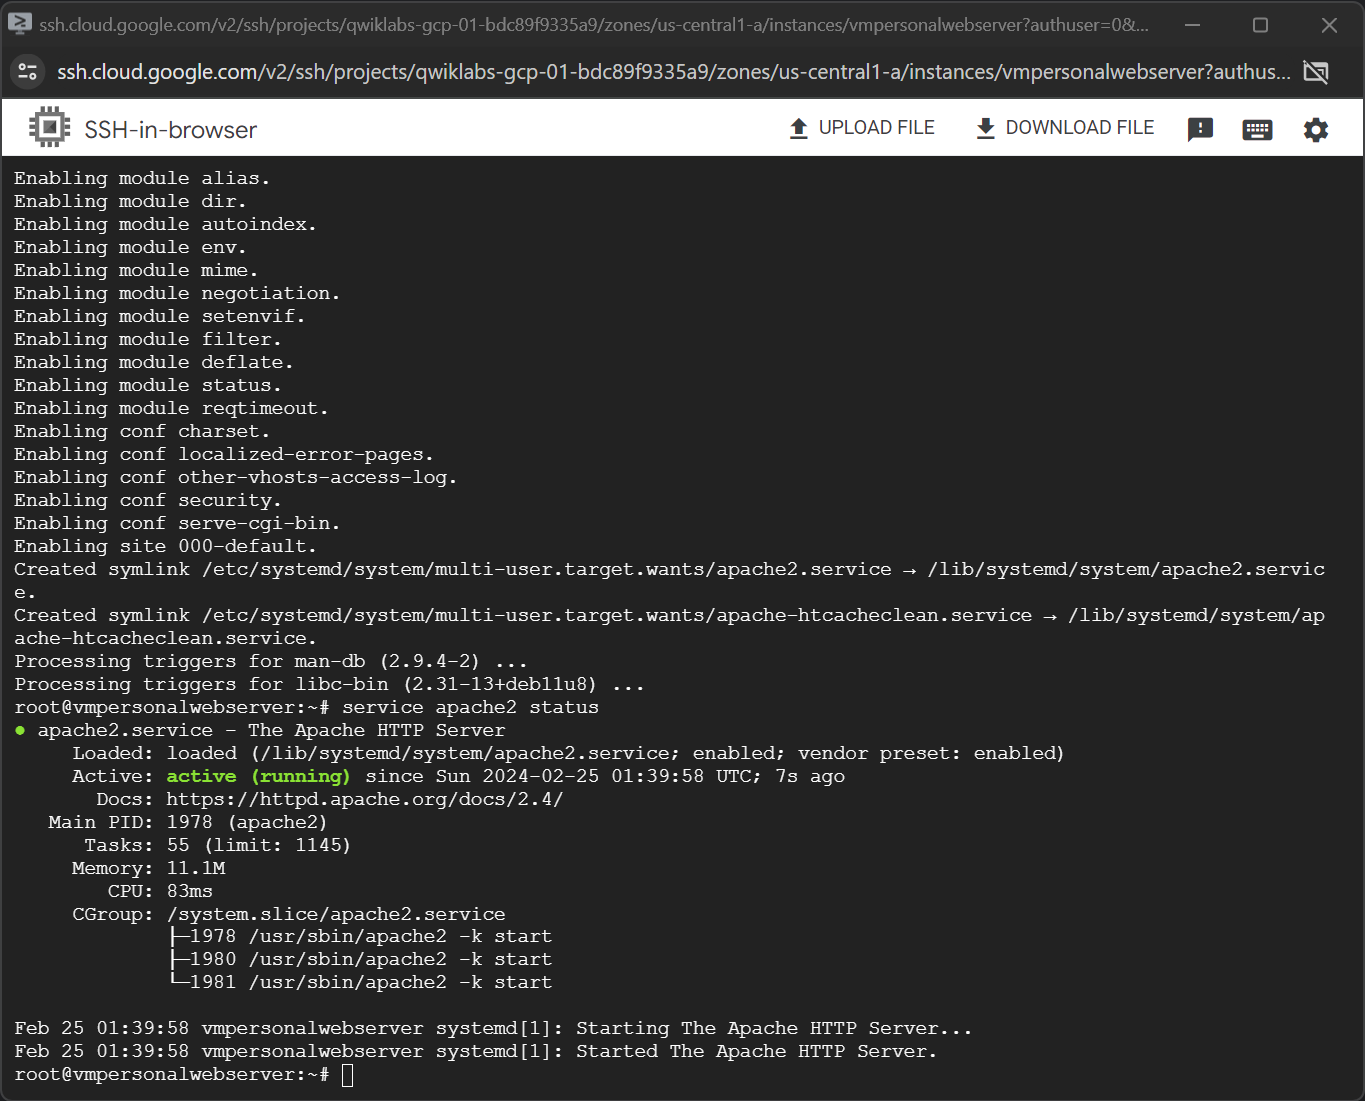
\includegraphics[width=1\linewidth]{M4_Servicios_Cómputo_en_la_Nube/Tarea_5_Creación_Máquinas_Virtuales_en_Nube/reporte/figuras/2_2_1_PHP_servidor_Web.png}
    \captionof{lstlisting}{Configuración del servidor web apache2}
    \label{fig:Google_3}
\end{figure}

\vspace{5em}

\subsection{Configuración de la Máquina Virtual para que sea pública}

Como establecimos al momento de habilitar la opciones de \textbf{Allow HTTP traffic} y \textbf{Allow HTTPS traffic} y al momento de configurar el servidor web apache2, ingresamos en una pestaña la dirección IP y observamos como a través de nuestro navegador web pudimos acceder a la visualización de la página web por defecto del servifor de apache2.

\begin{figure}[H]
    \centering
    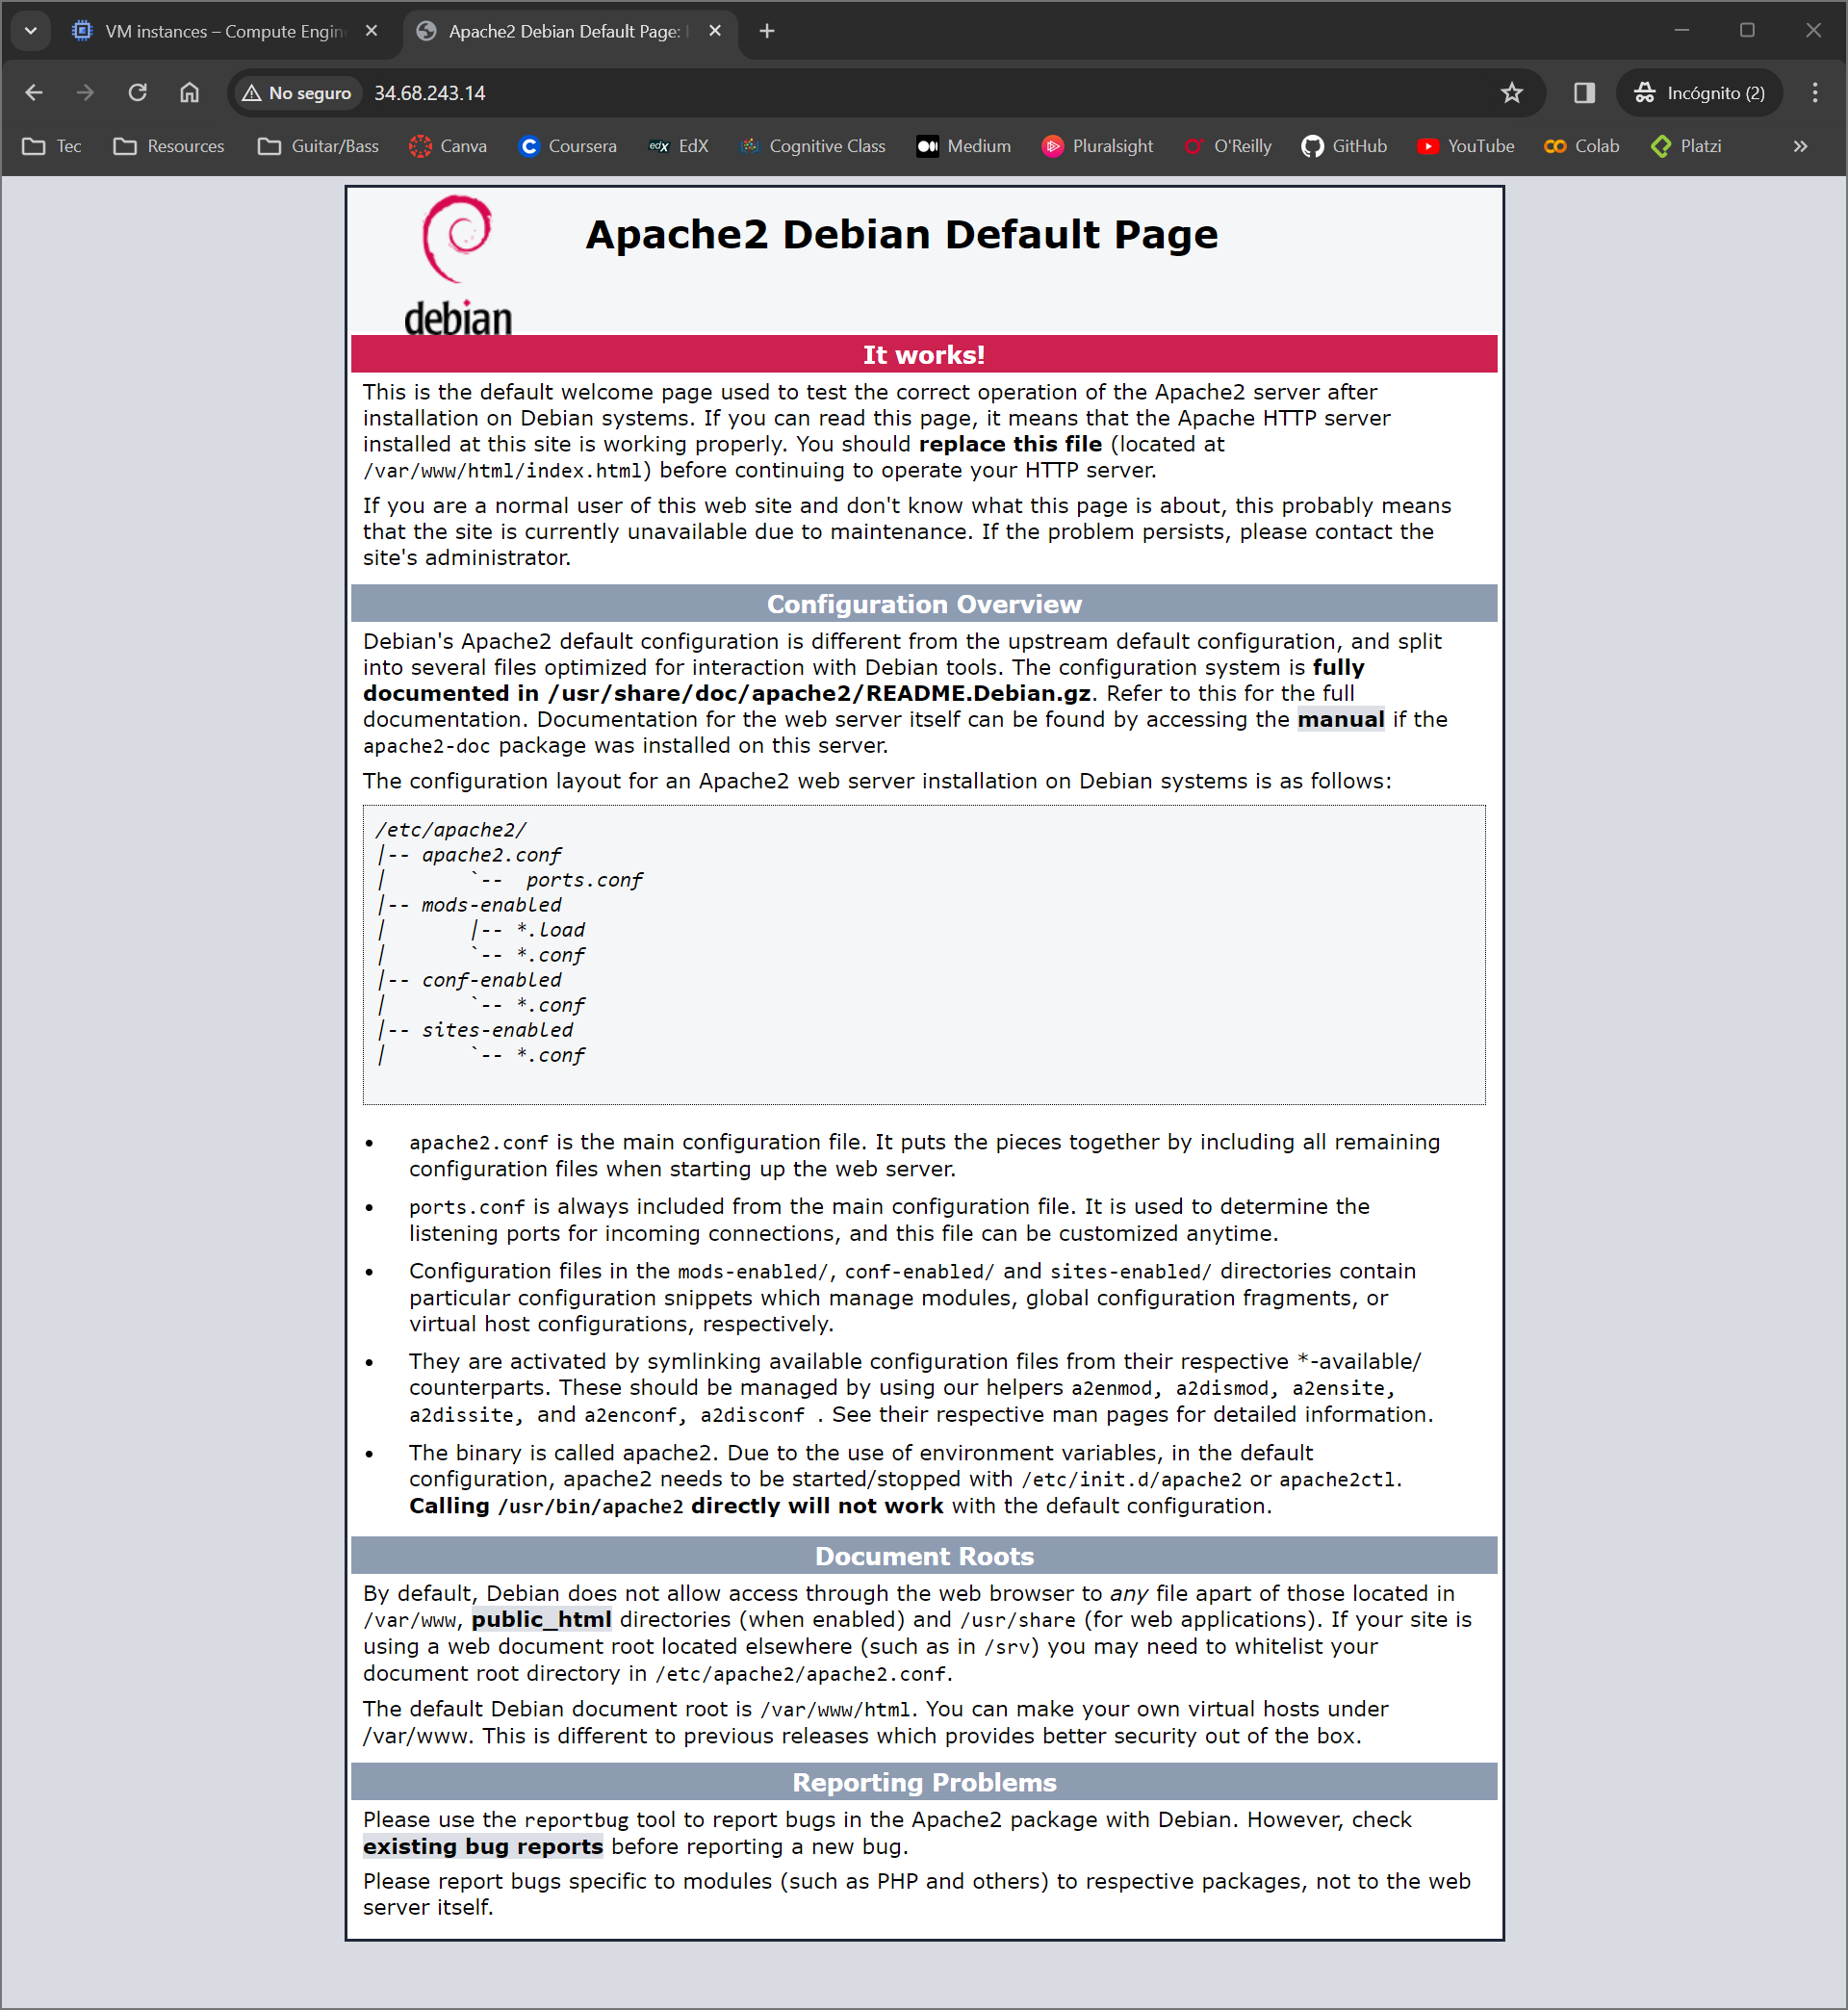
\includegraphics[width=1\linewidth]{M4_Servicios_Cómputo_en_la_Nube/Tarea_5_Creación_Máquinas_Virtuales_en_Nube/reporte/figuras/2_3_1_Configuración_Pública.png}
    \captionof{lstlisting}{MV como servidor web, página de apache por defecto}
    \label{fig:Google_4}
\end{figure}

Se intentó crear una llave \textbf{SSH-2 RSA} con la aplicación \textbf{PuttyGen} para posteriormente establecer la conexión y poder realizar la transferencia de archivos con la aplicación de FileZilla. Snn embargo, después de varios intentos y al no funcionar tuvimos que optar por la opción de generar los certificados (llaves SSH) y descargarlos a través de la misma consola shell de Google como se observa en la figura \ref{fig:Google_5}.


\begin{figure}[H]
    \centering
    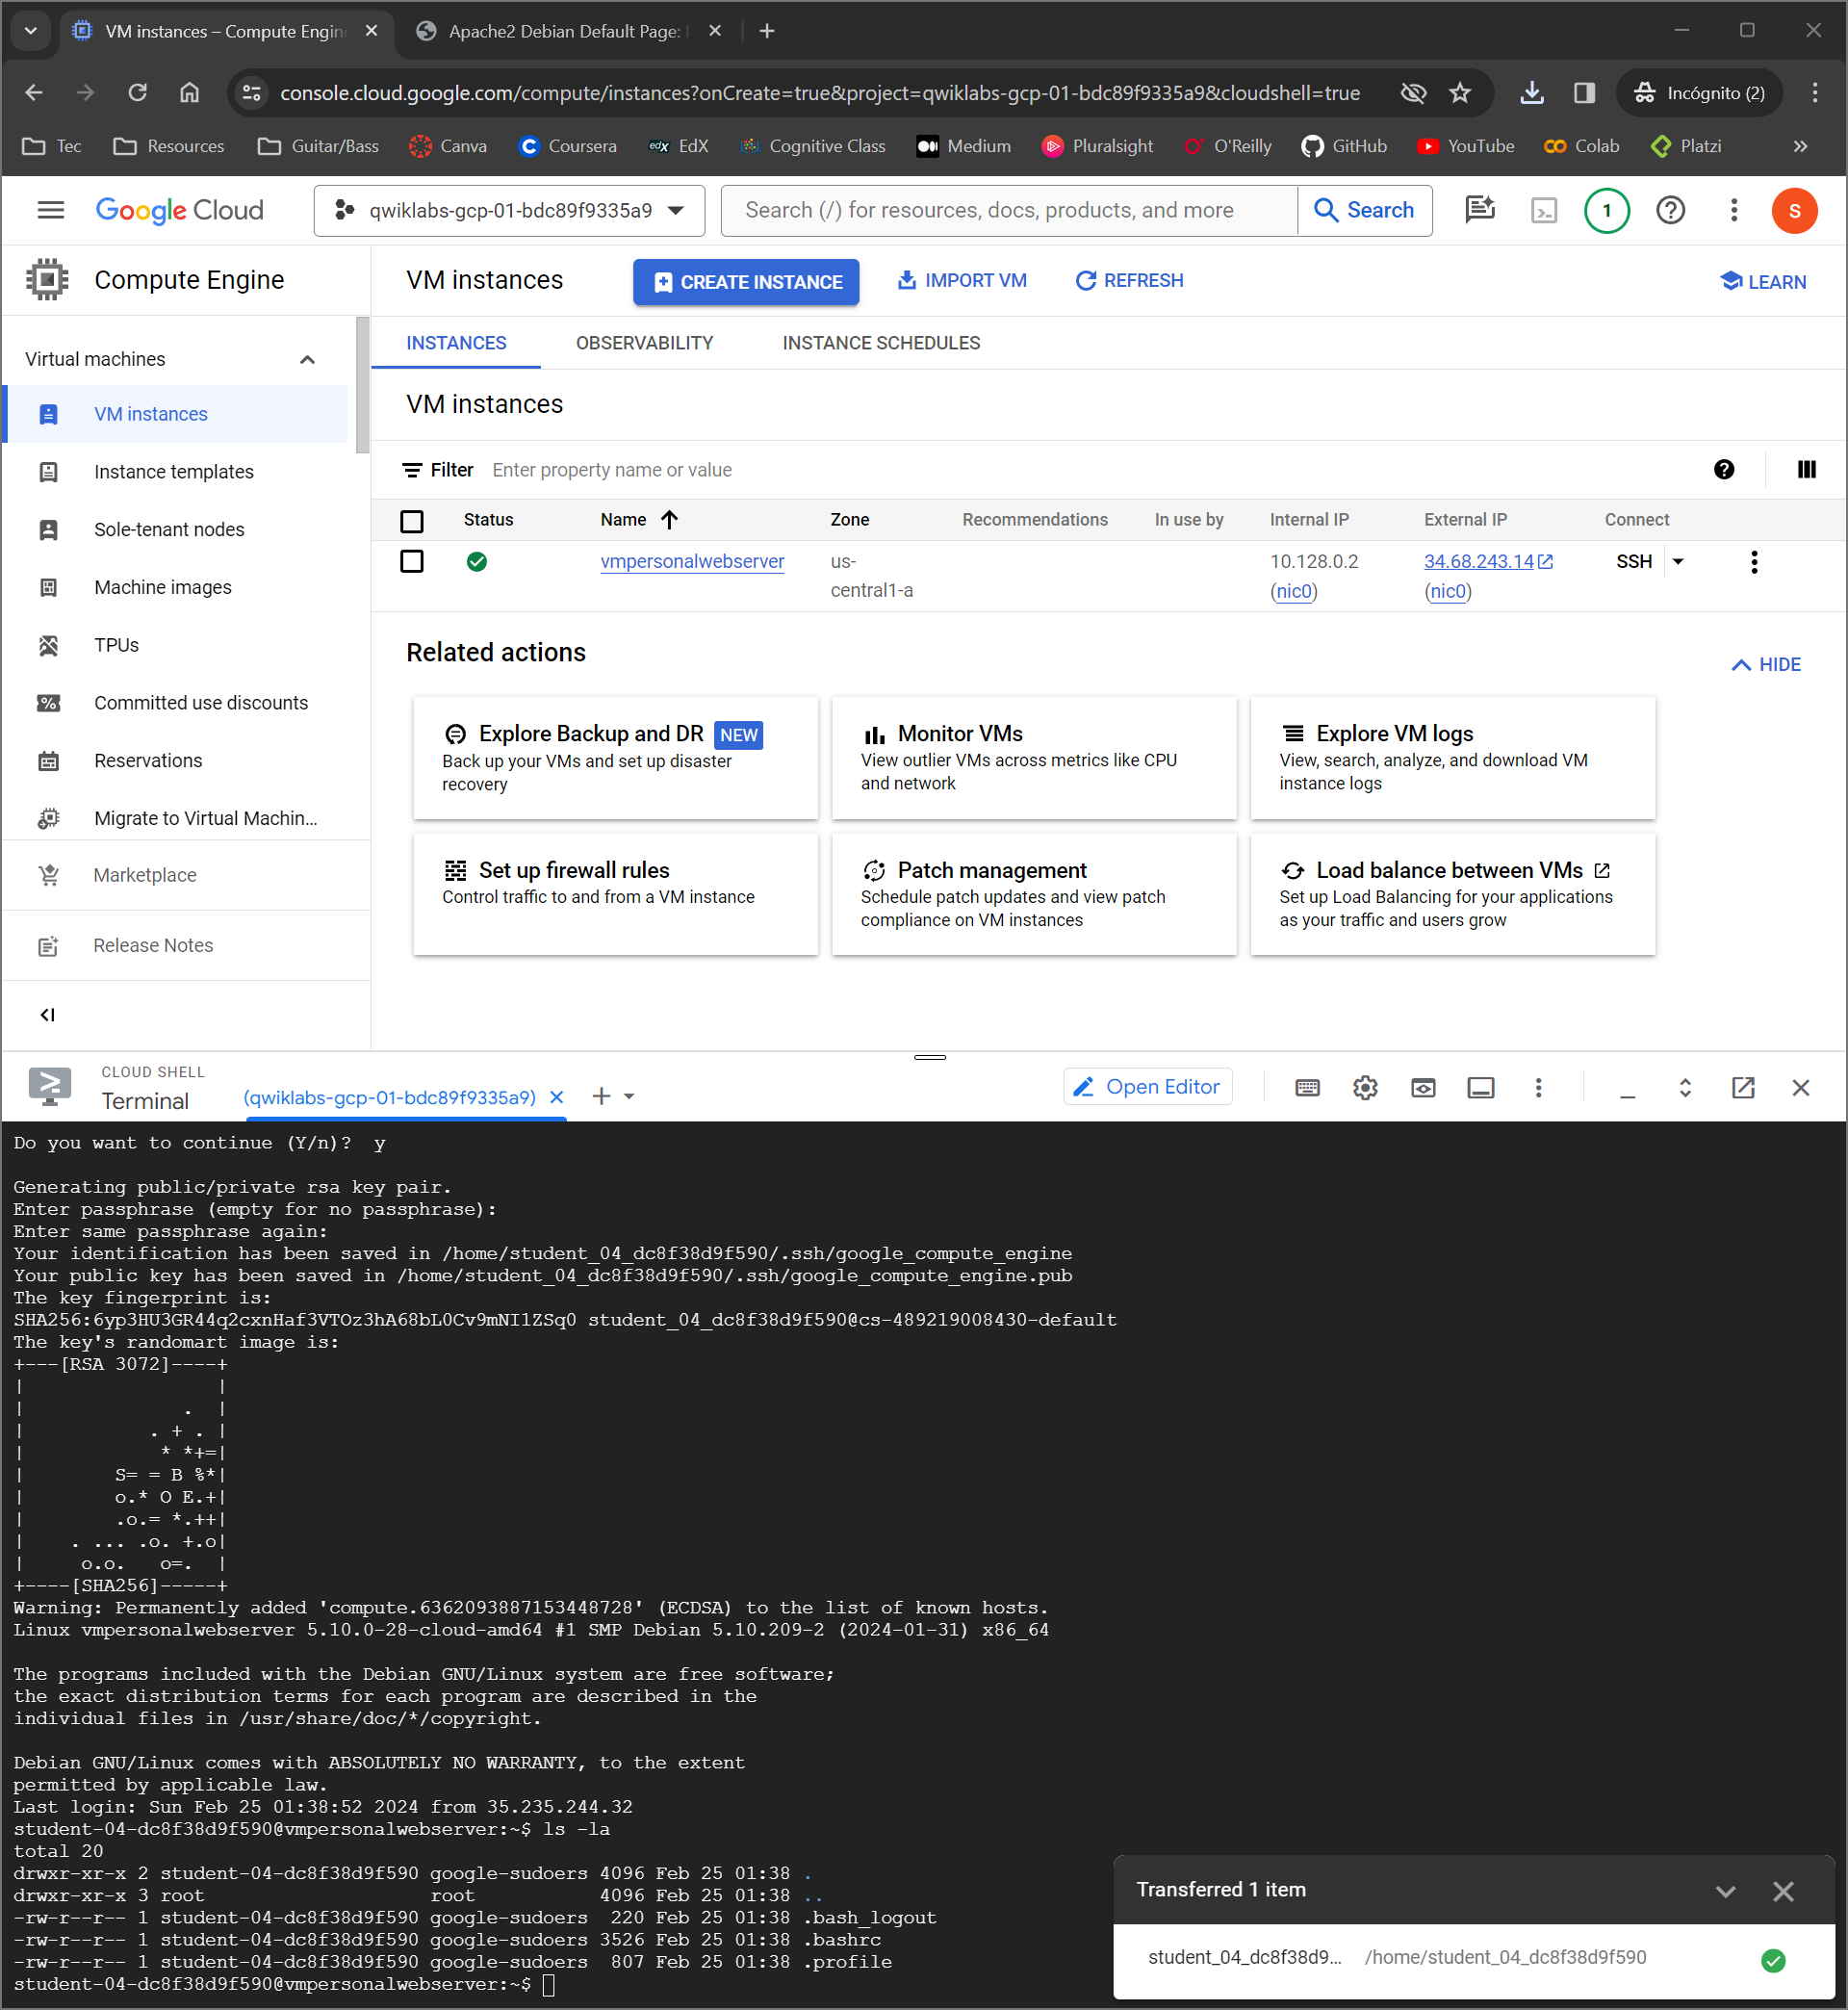
\includegraphics[width=1\linewidth]{M4_Servicios_Cómputo_en_la_Nube/Tarea_5_Creación_Máquinas_Virtuales_en_Nube/reporte/figuras/2_3_2_Configuración_Pública.png}
    \captionof{lstlisting}{Creación de llaves SSH}
    \label{fig:Google_5}
\end{figure}

\subsection{Carga de los archivos del sitio}

Posteriormente en FileZilla establecimos una nueva conexión cargando la llave que previamente habíamos descargado, en ese caso no tuvimos ya problema para establecer conexión con la Máquina Virtual. Un paso importante es que en la consola SSH de la Máquina Virtual ejecutamos el comando \textbf{chmod 777 /var/www/html} para de igual manera permitir la transferencia de archivos. En la figura \ref{fig:Google_6} podemos observar cómo la transferencia se realizó de forma exitosa.


\begin{figure}[H]
    \centering
    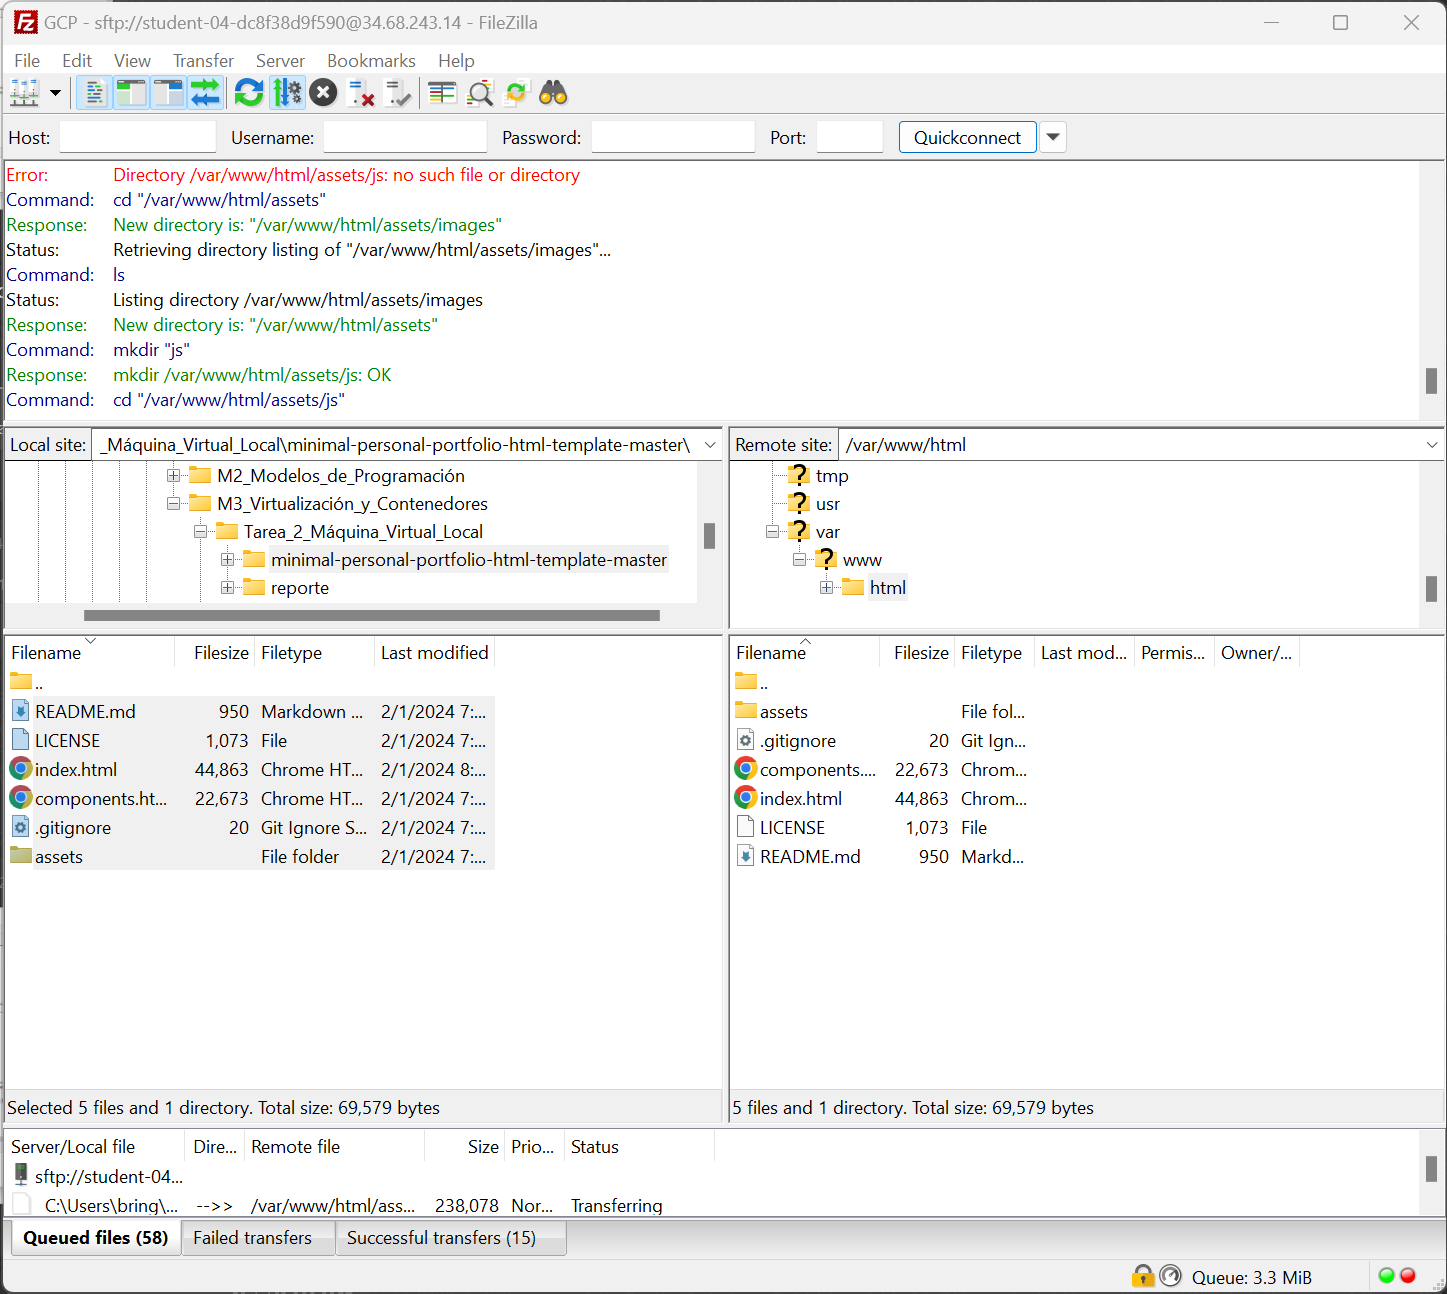
\includegraphics[width=1\linewidth]{M4_Servicios_Cómputo_en_la_Nube/Tarea_5_Creación_Máquinas_Virtuales_en_Nube/reporte/figuras/2_4_1_Carga_archivos.png}
    \captionof{lstlisting}{Transferencia de Archivos a Máquina Virtual de Google a través de FileZilla}
    \label{fig:Google_6}
\end{figure}

\vspace{5em}

Finalmente ingresamos en una nueva pestaña nuestra dirección IP externa \textbf{34.68.243.14} donde observamos que la página web que cargamos a nuestro servidor web se visualizó de forma correcta, por lo que la creación de la Máquina Virtual fue exitosa.

\begin{figure}[H]
    \centering
    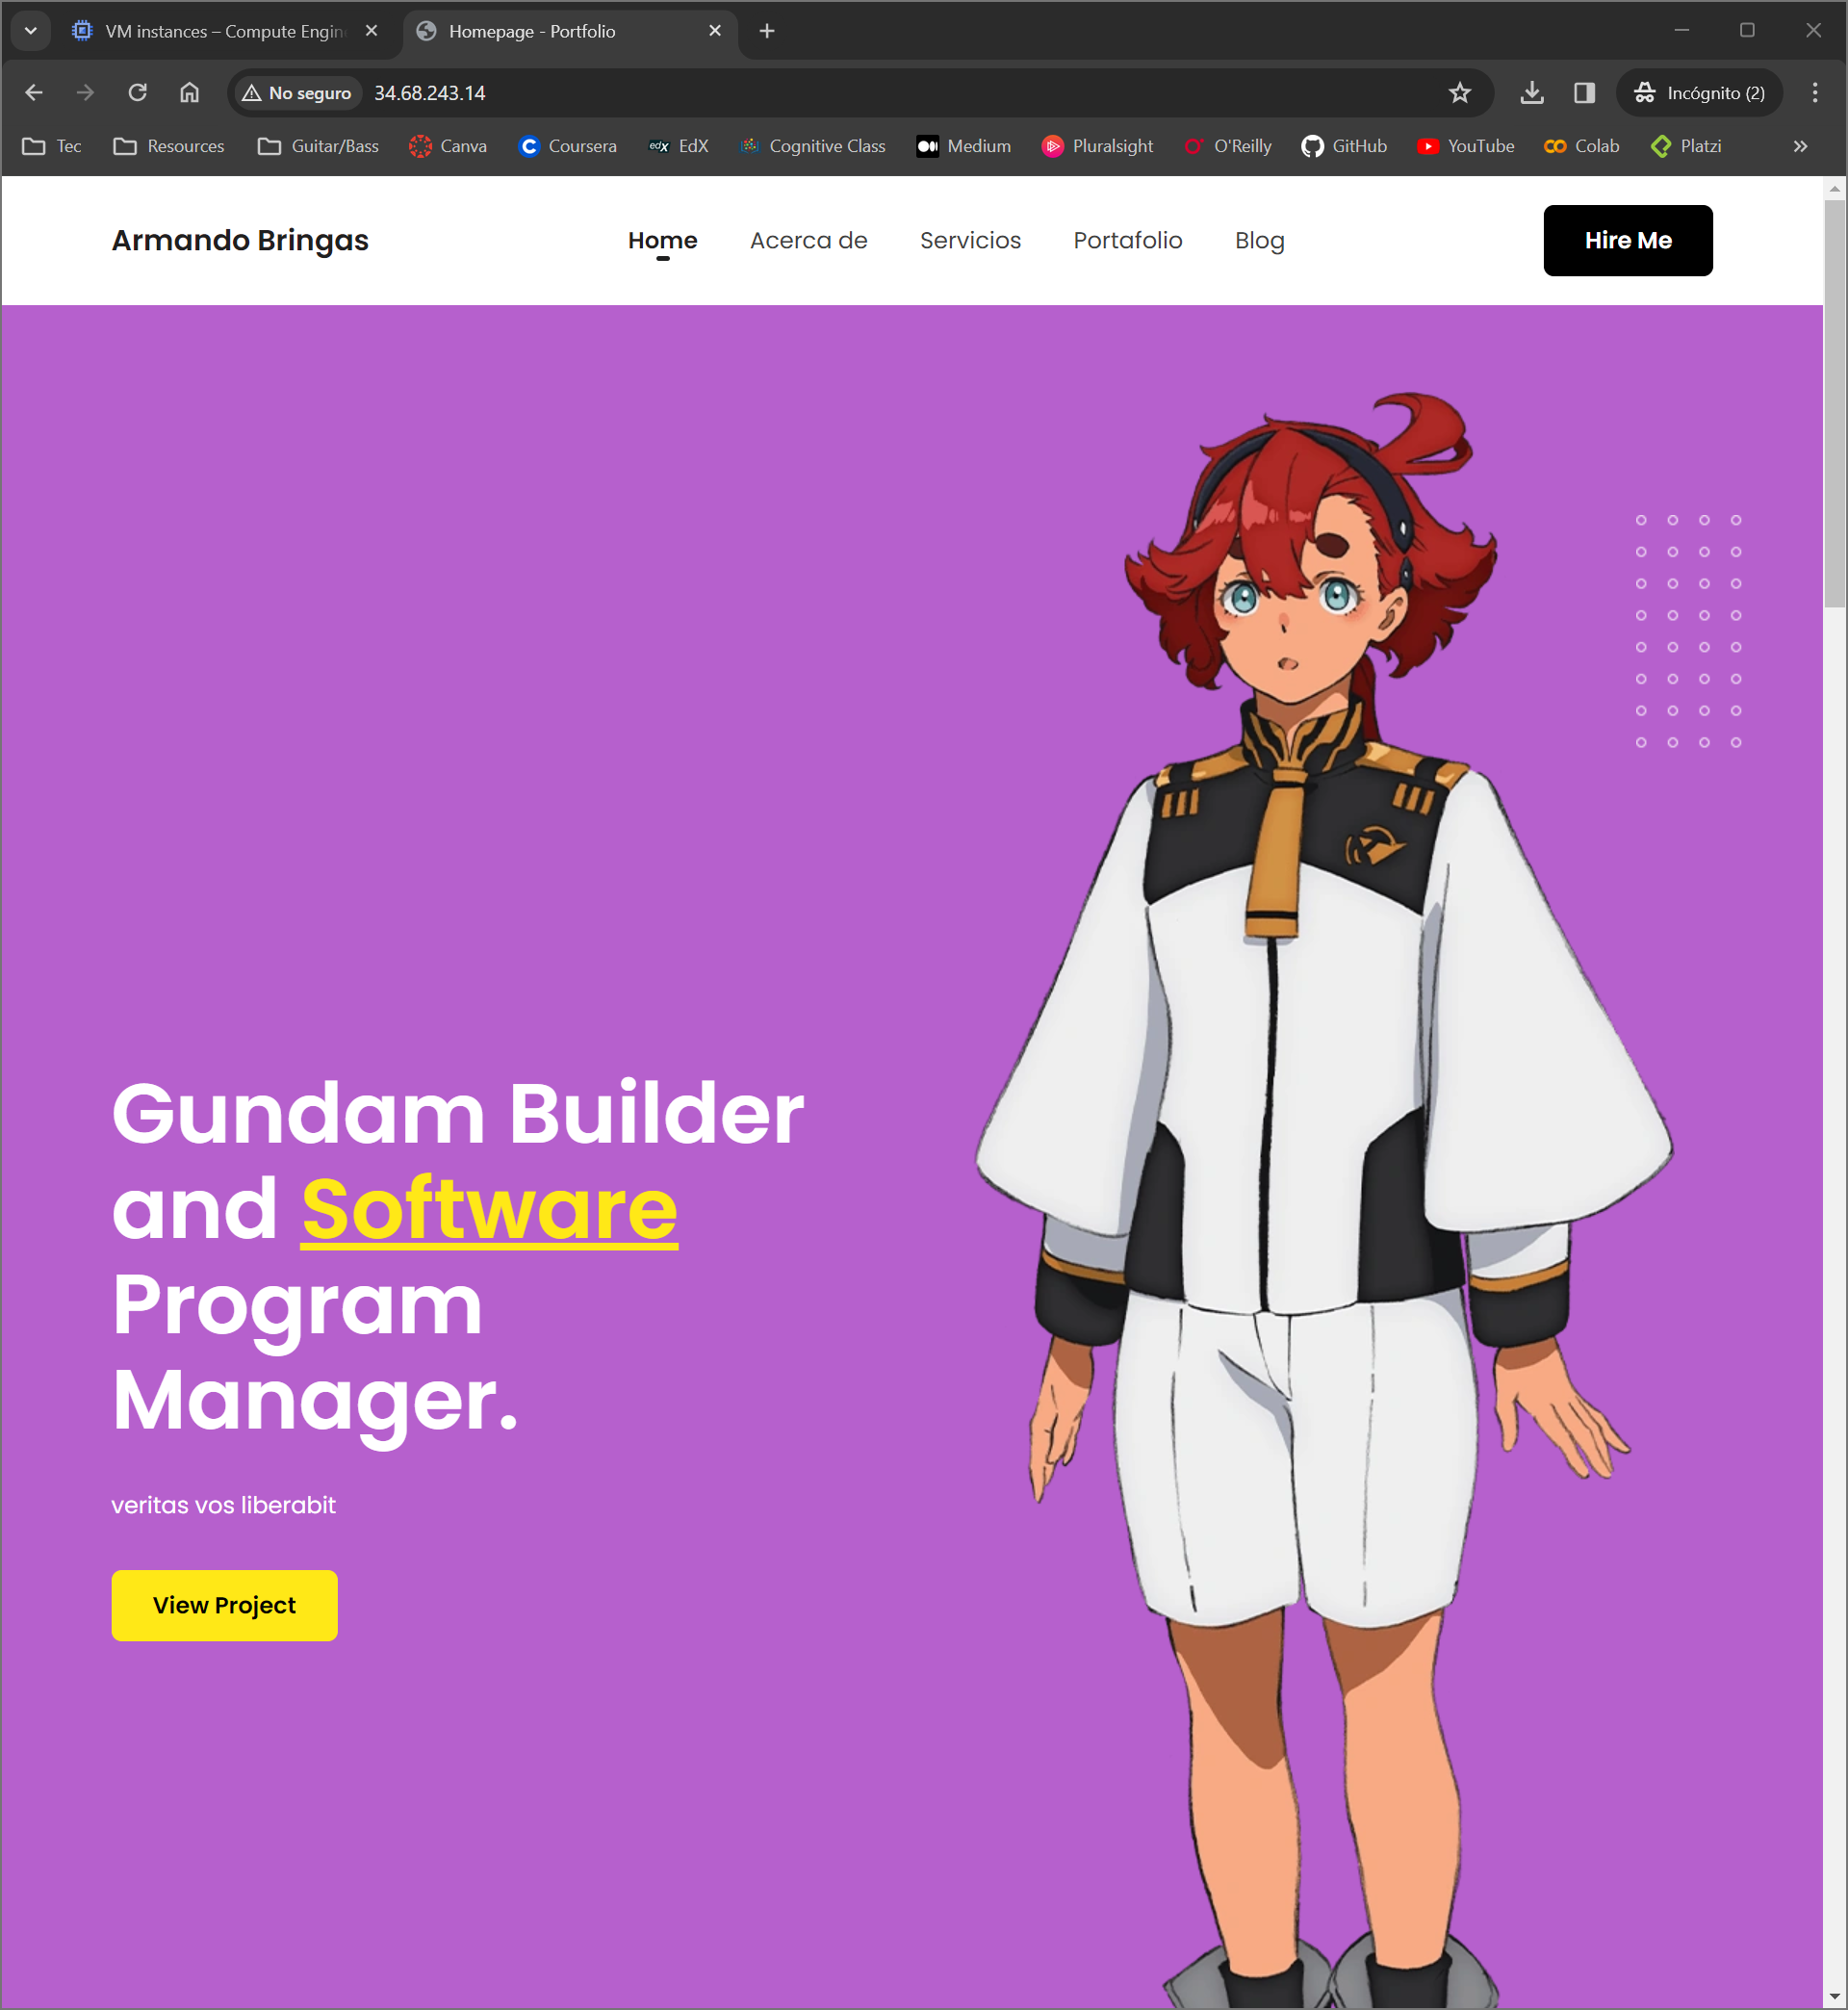
\includegraphics[width=1\linewidth]{M4_Servicios_Cómputo_en_la_Nube/Tarea_5_Creación_Máquinas_Virtuales_en_Nube/reporte/figuras/2_4_2_Carga_archivos.png}
    \captionof{lstlisting}{Visualización de la página web}
    \label{fig:Google_7}
\end{figure}

\vspace{5em}

\section{Reflexión de las Máquinas Virtuales en la nube}

En comparación de generar Máquinas Virtuales en un entorno local, vemos múltiples ventajas en hacerlas a través de un proveedor de servicios en la nube sobretodo con respecto al escalado vertical y horizontal de recursos, y al incluso aminorar costos OpeX con respecto a colocar nueva infraestructura para satisfacer la demanda de las nuevas necesidades si estás van siendo incrementales.

\vspace{1em}

Algo que nos pareció muy atractivo es que para cuando por ejemplo necesitamos montar un servidor web como el de la práctica podemos optar en los servicios en la nube por usar una máquina virtual que consuma pocos recursos y la menos costosa para satisfacer nuestras necesidades. Si vamos teniendo aplicaciones más demandantes podemos optar por escoger opciones con mayor capacidad.

\vspace{1em}

Por último, se nos facilitó más la creación y configuración de la Máquina Virtual en Azure, con Google Cloud la configuración fue más compleja por la capa de seguridad que agrega, de igual manera nos hubiera gustado experimentar con los comandos de Linux para cargar directamente los archivos en la Máquina Virtual, pero por cuestiones de tiempo en el laboratorio optamos en hacerlo a través de FileZilla. Aquí nuestra interrogante es si de acuerdo a lo anterior podríamos inferir que las Máquinas Virtuales de Google son más seguras, pero nos decantamos más en pensar que se trata más de una cuestión de preferencias de configuración y que ambos servicios garantizan un nivel similar de seguridad.





\end{document}